\section{Spectral Analysis}
In this chapter different way of analysing the spectrum will be covered. Also how it might be useful in the implementation of the transcription system will be considered.
\subsection{Spectral Centroid}
This chapter will show what the feature spectral centroid is.\\
The spectral centroid feature will calculate the center of gravity(COG) of a spectrum it is defined by the frequency weight power spectrum normalized by the unweigth sum \citep{ACA}:
\begin{equation}\label{Spectral Centroid eq}
	\upsilon_{SC}(n) = \frac{\displaystyle\sum_{k = 0}^{\frac{\kappa}{2-1}} k\vert X(k,n) \vert^2}{\displaystyle\sum_{k = 0}^{\frac{\kappa}{2-1}} \vert X(k,n) \vert^2 }    
\end{equation} 
However the spectral centroid can also be calculated using the magnitude spectrum instead of the power spectrum, with means the power is not taken in the calculation\citep{ACA}.
\\
The point found by the spectral centroid feature should correlate with the timbre dimension of how sharp or bright the sound is \citep{ACA}. 

\begin{figure}[h]
	\begin{center}
		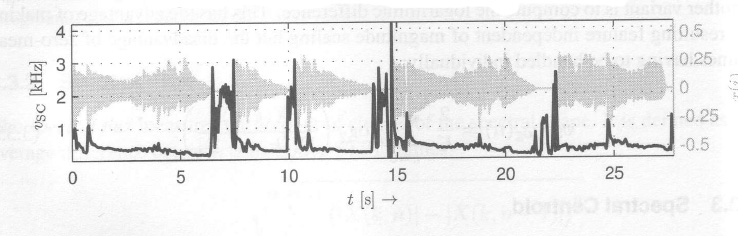
\includegraphics[scale = 0.5]{fig/spectral_centroid.jpg}
		\caption{Spectral Flux black = the Spectral centroid Gray = the sound \citep{ACA}}
		\label{Spectral centroid pic}
	\end{center}
\end{figure}

\\
This feature might be used in a transcription system because it should describe how sharp or bright a sound will sound, so this feature could be used to classify as sound. but there might be problems in the pauses/noise areas as seen on figure \ref{Spectral centroid pic} as there is a high peak at some of the pauses. 
\subsection{Spectral Rolloff}
This chapter will explain what the spectral rolloff is.\\
The Spectral Rolloff is defined as the frequency bin at which the magnitude of the STFT reaches a percentage K of the overall sum of magnitudes, can be calculated like\citep{ACA}\\
\begin{equation}\label{ eq:normal spectral rolloff}
	\upsilon_{SR}(n) = i \vert _{\displaystyle\sum_{k = 0}^i \vert X(k, n) \vert = K  \displaystyle\sum_{k = 0}^ {\frac{\kappa}{2-1}}\vert X(k, n) \vert}
\end{equation}
\\
Normal the value for K is around 0.85 or 0.95. Low results indicates insufficient magnitudes components at high frequencies and the a low audio bandwidth\citep{ACA}.\\
Different ways to compute the spectral rolloff can be that only parts of the spectral energy is taken into considerations that is done by use an fmin and a fmax\citep{ACA}
\begin{equation}\label{ eq: fmin and fmax spectral rolloff}
	\upsilon_{SR, \Delta f}(n) = i \vert _{\displaystyle\sum_{k = k(f_{min})}^i \vert X(k, n) \vert = K \displaystyle\sum_{k = k_(f_{min})}^ {k(f_{max})}\vert X(k, n) \vert}
\end{equation}
It can also be common to use the power spectrum
\begin{equation}\label{ eq:power spectral rolloff}
	\upsilon_{SR}(n) = i \vert _{\displaystyle\sum_{\kappa = 0}^i \vert X(\kappa, n) \vert^2 = \kappa * \displaystyle\sum_{\kappa = 0}^ {\frac{K}{2-1}}\vert X(\kappa, n) \vert^2}
\end{equation}

\\
For our project the spectral rolloff could be used to determine the sound in the classification. 

\begin{figure}[h]
	\begin{center}
		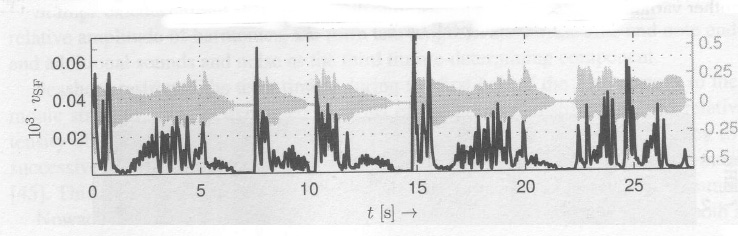
\includegraphics[scale = 0.5]{fig/spectral_rolloff.jpg}
		\caption{Spectral Flux black = the Spectral rolloff Gray = the sound \citep{ACA}}
		\label{Spectral rolloff pic}
	\end{center}
\end{figure}
for our project the spectral rolloff could also be used to determine the sound in the classification, as the spectral rolloff will tell about the roughness of the sound. 


\subsection{Spectral Flux}
This chapter will explain the feature Spectral Flux and its uses.\\
The spectral Flux is how much the spectrum shape change between the different frames it can be defined as\citep{ACA}:
\begin{equation}\label{Spectral Flux eq}
	\upsilon_{SF}(n) = \frac{\sqrt{\displaystyle\sum_{\kappa=0}^{K/2-1}(\vert X(\kappa,n\vert-\vert X(\kappa,n-1)\vert)^2}}{K/2}
\end{equation} 
The spectral flux feature can be described as a representation of the roughness of a sound. The result that one will get from a spectral flux feature is in the range from 0 to A where A is the maximum magnitude possible in the spectrum\citep{ACA}. when looking at spectral flux in a signal it will be flat at silence and spike at pitch changes\citep{ACA}.
\begin{figure}[h]
	\begin{center}
		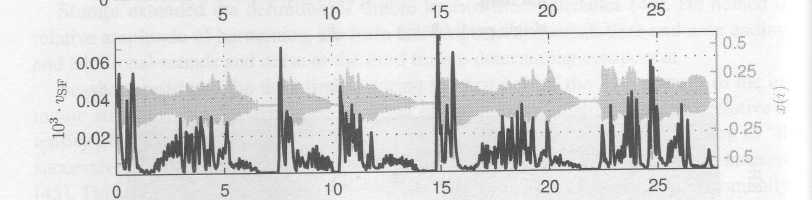
\includegraphics[scale = 0.5]{fig/spectral_flux.jpg}
		\caption{Spectral Flux black = the Spectral Flux Gray = the sound \citep{ACA}}
		\label{Spectral flux pic}
	\end{center}
\end{figure}
For use in note onset detection (finding the start of the note) only an increase in the spectral energy is wanted an one can consider using a different way to calculate the spectral flux\citep{ACA}:
\begin{equation}
	\upsilon_{SF}(n) = \vert X(\kappa,n)\vert-\vert X(\kappa,n-1)\vert
\end{equation}
When doing this all negative values has to be set to zero so that only increase is detected\citep{ACA}.
\\
For a transcription system the spectral flux as described can be considered to do the segmentation of a sound signal because it can detect an onset. 
 
\subsection{Spectral Slope}
This chapter will be on explaining what the spectral slop feature is.\\
The spectral slope as the name indicate is a feature that is a measure of the slop in the spectral energy\citep{ACA}. The spectral slope is calculated using a linear regression of the spectral magnitude spectral, the slop is then estimated using this equation\citep{ACA}
\begin{equation}
	\upsilon _{SSI} (n) = \frac{\displaystyle\sum_{\kappa = 0}^{K/2-1}(\kappa - \mu_\kappa)(\vert X(\kappa,n) - \vert - \mu_\vert X \vert)}{\displaystyle\sum_{\kappa = 0}^{K/2-1}(\kappa - \mu_\kappa)^2}
\end{equation}
\begin{equation}
	= \frac{\displaystyle\sum_{\kappa = 0}^{K/2-1}\kappa X(\kappa,n) - \displaystyle\sum_{\kappa = 0}^{K/2-1}\kappa\displaystyle\sum_{\kappa = 0}^{K/2-1}\vert X(\kappa,n)\vert}{K \displaystyle\sum_{\kappa = 0}^{K/2-1}\kappa^2-(\displaystyle\sum_{\kappa = 0}^{K/2-1}k)^2}
\end{equation}
The result the one can get from these equations is defined by range of the spectral magnitude.
\begin{figure}[h]
	\begin{center}
		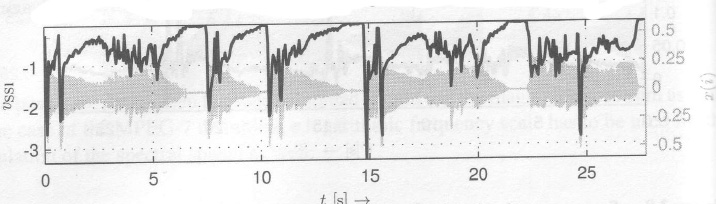
\includegraphics[scale = 0.5]{fig/spectral_slope_fig.jpg}
		\caption{Spectral slope black = the Spectral slope Gray = the sound \citep{ACA}}
		\label{Spectral slope pic}
	\end{center}
\end{figure}
As it is possible to see on the picture of the spectral slope (fig \ref{Spectral slope pic}) one use for this feature could be in the segmentation, because in the silent or the part with just it is high and when there is a signal is goes down. 
